
%%*************************************************************************
%%
%% Analysis of Biosignals by Biologically Inspired Algorithms
%% V1.0
%% 2011/05/05
%% by Peter Boraros
%% See:
%% http://www.pborky.sk/contact
%% for current contact information.
%%
%% Desription goes here.
%%
%%
%%*************************************************************************
%% Legal Notice:
%%
%% This code is offered as-is without any warranty either expressed or
%% implied; without even the implied warranty of MERCHANTABILITY or
%% FITNESS FOR A PARTICULAR PURPOSE! 
%% User assumes all risk.
%%
%% This work by Peter Boraros is licensed under a 
%% Creative Commons Attribution-NonCommercial-ShareAlike 3.0 Unported License.
%% http://creativecommons.org/licenses/by-nc-sa/3.0/


\documentclass[a4paper]{IEEEtran}

\usepackage{cite}
% \usepackage[nocompress]{cite}
\usepackage{ifpdf}

\ifpdf
\usepackage[pdftex]{graphicx}
\graphicspath{{./img/}}
\DeclareGraphicsExtensions{.pdf}
\else
\usepackage[dvips]{graphicx}
\graphicspath{{./img/}}
\DeclareGraphicsExtensions{.eps}
\fi

\usepackage[cmex10]{amsmath}
\usepackage{amsfonts}
\usepackage{amssymb}
\interdisplaylinepenalty=2500

\usepackage{algorithmic}

\usepackage{array}

\usepackage{mdwmath}
\usepackage{mdwtab}

\usepackage{eqparbox}

% \usepackage[tight,normalsize,sf,SF]{subfigure}
\usepackage[tight,footnotesize]{subfigure}

% \usepackage[caption=false,font=normalsize,labelfont=sf,textfont=sf]{subfig}
% \usepackage[caption=false,font=footnotesize]{subfig}

\usepackage[utf8x]{inputenc}
\usepackage{url}
\usepackage{fixltx2e}
\usepackage{stfloats}
\usepackage{ucs}

% correct bad hyphenation here
\hyphenation{op-tical net-works semi-conduc-tor}

% IEEEtran contains the IEEEeqnarray family of commands that can be used to
% generate multiline equations as well as matrices, tables, etc., of high
% quality.

% stfloats.sty was written by Sigitas Tolusis. This package gives LaTeX2e
% the ability to do double column floats at the bottom of the page as well
% as the top. (e.g., "\begin{figure*}[!b]" is not normally possible in
% LaTeX2e). It also provides a command:
%\fnbelowfloat
% to enable the placement of footnotes below bottom floats (the standard
% LaTeX2e kernel puts them above bottom floats). This is an invasive package
% which rewrites many portions of the LaTeX2e float routines. It may not work
% with other packages that modify the LaTeX2e float routines. The latest
% version and documentation can be obtained at:
% http://www.ctan.org/tex-archive/macros/latex/contrib/sttools/
% Documentation is contained in the stfloats.sty comments as well as in the
% presfull.pdf file. Do not use the stfloats baselinefloat ability as IEEE
% does not allow \baselineskip to stretch. Authors submitting work to the
% IEEE should note that IEEE rarely uses double column equations and
% that authors should try to avoid such use. Do not be tempted to use the
% cuted.sty or midfloat.sty packages (also by Sigitas Tolusis) as IEEE does
% not format its papers in such ways.


\begin{document}
\title{Analysis of biosignals by means of\\ biologically inspired algorithms}

\author{Peter~Boraros% <-this % stops a space
%\IEEEcompsocitemizethanks{
%	\IEEEcompsocthanksitem P. Boraros is with Department of Cybernetics, 
%		Czech Technical University, Prague, Czech Republic.\protect\\
%		E-mail: see http://www.pborky.sk/contact}
}



% The paper headers
\markboth{Peter Boraros, Czech technical university, Faculty of Electrical Engineering,
Prague, Czech Republic}%
{Shell \MakeLowercase{\textit{et al.}}: Bare Demo of IEEEtran.cls for Computer Society Journals}

\IEEEcompsoctitleabstractindextext{%
\begin{abstract}
The aim of this document is to show the usage of biologically inspired algorithms
in analysis of facial electromyography and electroencephalography.
Concretelly, it depicts the process of obtaining data, preprocessing using fast fourier
transform and classifing by means of self-organizing maps. 
Searching through the parameter space in order to find proper parametrisation of whole
classification process is performed by genetic algorithm.
\end{abstract}}

\maketitle
\IEEEdisplaynotcompsoctitleabstractindextext
\IEEEpeerreviewmaketitle


\section{Introduction}
\IEEEPARstart{S}{submission} to this work is to implement methods for analysis 
electromyography (EMG) and electroencephalography (EEG) 
signals in order to allow estimation of the subject`s mimics, 
feelings or enable ability to classify the sleep stages and possibly control 
external equipment during specific sleep stage.

This work depicts usage of self-organizing maps (SOM) as well the usage of genetic
algorithm. It ispossible to use other recognition techniques but usage of mentioned 
methods was induced by semestral work in school.

%TODO: used methods

%Software used by this available at \url{https://github.com/pborky/biosiglab}.

\section{Description}
\subsection{Training data, preprocessing}
Training data is pulse-code modulated (PCM) signal as well the classification 
information attached during the signal gathering.
PCM signal is single channel balanced measure of voltage
quantized at 24-bit sample size
and sampled at frequency 4kHz. To search for optimal sampling frequency,
it is reduced by averaging particular number of samples. Classification
is reduced by electing most frequent classes.

Signal is then choped into overlaping slices (windows).
Mean of each slice is subtracted.
Signal has to be transformed from time domain to frequency domain.
This can be achieved by fourier or wavelet transform.
Wavelet transform captures not only a notion of the frequency content of the input,
by examining it at different scales, but also temporal content.
This document describes only fast fourier transform.
Fast fourier transform is aplied to each slice resulting in
complex spectral components of same size like time windows.
Phase information should be discarded.

Next the resulting vectors are subject to reduction by masking its components.
This is frequency filtering.

Spectral components are subject to normalisation.
There are several algorithms to choose. Best seems to be 
discrete histogram or logistic equlization with scaling the values between [0, 1].
Other possibilities are logaritmic or range normalisation, that again normalize
values between [0, 1].

Sampling frequency, window size, overlap, frequency filters and normalisation algorithm 
are parameters that to be sought.

\subsection{Self-organizing map}
Self-organising map is method of vector quantisation that can be used to 
cluster analysis. Clusters are represented by best matching units (BMUs)
- vectors that are conected in topological structure. Their value is calculated
by iterative process using training data. Topological neighborhood plays 
also important role and it distincts this method from k-means cluster analysis.
After iterations BMUs should represent real clusters in data.

This unsupervised process can be turned to supervised by adding a classification
information before process.
Class information  could be encoded with 1-of-N encoding and appended to the 
spectral vectors. After training it is removed from BMUs and class is 
decoded from 1-of-N code as maximal component of appended part.

The spatial 
layout of topological surface has to be checked. It should not contain irregularites, 
the surface should be 'plain' and it should follow the data and the clusters.
To quantify this criterion tolopological error is defined. It is the proportion 
of all data vectors for which first and second BMUs are not adjacent units.

Another criterion is validation/testing error. Traning set is divided into k-folds
and using k-fold crossvalidation the map is trained using k-1 folds and  error 
is determined using the remaining fold. This is repeated for each fold. Average error is 
the subject to minimize. The value of \textit{k} was choosen: $ k = 3 $.
%TODO: link to more detailed descprition

Normalised data is then used to train the SOM, i.e. find the BMUs for given data.
The quality of output is controled by several parameters. The most important are 
training algorithm, maps size and topografic layout and lattice.

More detailed information about used algorithms is available at \cite{somtoolbox}.

\subsection{Search for the proper parameters}
Parameter space is searched for a best solution. There was identified
following degrees of freedom:
\begin{itemize}
	\item sampling frequency $ f_{samp} $,
	\item time window before fourier transform $ n_w $,
	\item overlap of time windows $ n_o $,
	\item frequency filter after fourier tranform ( interval $ (f_l, f_h) $ defines 
	range that is kept,
	\item normalisation method (histogram, logaritmic, range, logistic),
	\item SOM training algorithm (batch or sequential),
	\item lattice of SOM (hexagonal or rectangular),
	\item size of SOM (depend on size of traning dataset).
\end{itemize}
The search space is discrete, and the states are selected with prior knowledge.
Values of particular degrees of freedom are listed  in table \ref{searchspace}.


% TODO tabular list of degrees of freedom and search space
\begin{table}[h]
\caption{Search space}
	\begin{center}
		\begin{tabular}{|l| l |}
			\hline
			degree of freedom & values \\
			\hline
			\hline
			$ f_{samp} [Hz] $ & 256, 666, 1333, 4000\\
			\hline
			$ n_w $ & 80, 200, 800, 2000 \\
			\hline
			$ n_o $ & 2, 8 \\
			\hline
			$ (f_l[Hz], f_h[Hz]) $ & $ (0, 50) $,  $ (20, 250) $  \\
			\hline
			normalisation & histogram, logaritmic, range, logistic \\
			\hline
			training algorithm & batch, sequential  \\
			\hline
			map lattice & hexagonal, rectangular \\
			\hline
			map size  & small, normal \\
			\hline
		\end{tabular}
	\end{center}
\label{searchspace}
\end{table}

Possible optimalisation objectives are:
\begin{itemize}
	\item validation error $ e_v $ of the trained SOM network evaluated by k-fold
	crossvalidation, $ e_v \in \langle 0, 1 \rangle $,
	\item topological error $ e_t $ (should be zero),
	\item mean quantisation error $ e_q $,
	\item window size $ \Delta t_w $ (should be low in order to allow fast response times),
	\item running time $ t_r $ of whole process (not more than 20 seconds).
\end{itemize}

The fitness function was choosen empirically as follows:
\[ f = -\ln(e_v+10^{-4}) - \ln(\Delta t_w+\frac{1}{2}) - \ln(e_t+\frac{1}{2}) - P(t_r) \]
where:\\
$ P(t) $ is sigmoid function defined as:
\[ P(t) = \frac{5}{1+10\cdot e^{6-0.15t}} \]
$ e_v $ is validation error,\\
$ e_t $ is topological error,\\
$ t_r $ is running time,\\
$ \Delta t_w $ is window time span and it can be expressed as 
\[  \Delta t_w = \frac{n_w}{f_{samp}}  \]
where:\\
$ n_w $ is number of samples in window,\\
$ f_{samp} $ is sampling frequency.
%TODO: explain fitness function

\subsection{Genetic algorithm}
%TODO: rewrite
The whole process can be parametrised by several parameters. Optimal parametrisation 
is that maximizes correctness.
The considered objectives are validation error, size of window and overlap, 
computing time, etc.
The parameters can be determined by way of searching the search space. 
This document describes usage of genetic algorithm.

Genetic algorithm is inspired by nature and process of evolution.
It uses operators like selection, crossover, mutations. 
The search process by genetic algorithm is stochastic.
Further information on genetic algorithms can be obtained at \cite{ga,gawiki}.
%TODO: link to proof how and why it works

Implementation of genetic algorithm to be introduced has following properties:
\begin{itemize}
	\item given population size,
	\item random uniform initialization,
	\item selection strategy:
	\begin{itemize}
		\item surviving species are selected using stochastic universal 
		sampling reducing 
		the population size to given value,
	\end{itemize}
	\item crossover:
	\begin{itemize}
		\item parents for crossover are selected using fitness proportionate
		selection of the surviving species,
		\item count of selection rounds is determined by empiric formula
		\[ n_{pr} = \lceil 0.2\cdot n_{survived} \rceil \] 		
		where $ n_{survived} $ is the number of survived species after stochastic selection.
		The value of $ n_{pr} $ limits the count of selected species.
		\item for each parent, its pair is selected by random,
		\item genes selected by random are swapped; accepted solution is that 
		produces  offsprings different from parents (i.e. at least one differing gene must be
		kept),
	\end{itemize}
	\item mutations:
	\begin{itemize}
		\item species are selected by 2 ways:
		\begin{itemize}
			\item using inversed-fitness proportionate
			selection of the surving species where inverse fitness $ f' $ is 
			calculated using formula \[  f' = e^{-f} \]
			and count of selection rounds is
			\[ n_{mr} = \lceil \dfrac{0.1}{10\cdot e^{0.15\cdot i_{epoch} - 9}} 
			\cdot n_{survived} \rceil \]
			where: $ i_{epoch} $ is the actual epoch.
			The value of $ n_{mr} $ limits the count of selected species.
			\item from offsprings with probability to be selected for each one:
			\[ P_{mo} = \dfrac{0.3}{1+10\cdot e^{0.15\cdot i_{epoch} - 9}} \]
		\end{itemize}
		\item each bit is flipped with probability\\
		\[ P_{mb} = \dfrac{0.3}{1+50\cdot e^{-0.4\cdot i_{epoch}}} \]
	\end{itemize}
	\item stop condition:
	\begin{itemize}
		\item fitness of best-fit species for given interval of epochs has not changed.
	\end{itemize}
	
\end{itemize}
%TODO: further decritption

\section{Experiments}
\subsection{Training data}
Equipment used for this experiments is {Nia game controller}, made by 
{OCZ Techologies}. This device provides HID standard interface.
After it is connected, it starts to send 24-bit PCM samples, 
sampled at frequency 4kHz. The device has only one balanced channel, thus 
it is not possible to preform complex analysis of neural signals,
however for detection of EMG signal it is sufficient.

Training information is attached during data gathering by human operator 
through GUI application.
The PCM data from device is saved along with class information from
user interface.

Training data contains features of facial mimics.
Four class of grimaces was recorded: eye-wink (left, right, both), 
relax (no grimace).
Recording time is about 120 seconds.

\subsection{Self-organizing map}
\begin{figure}[h]
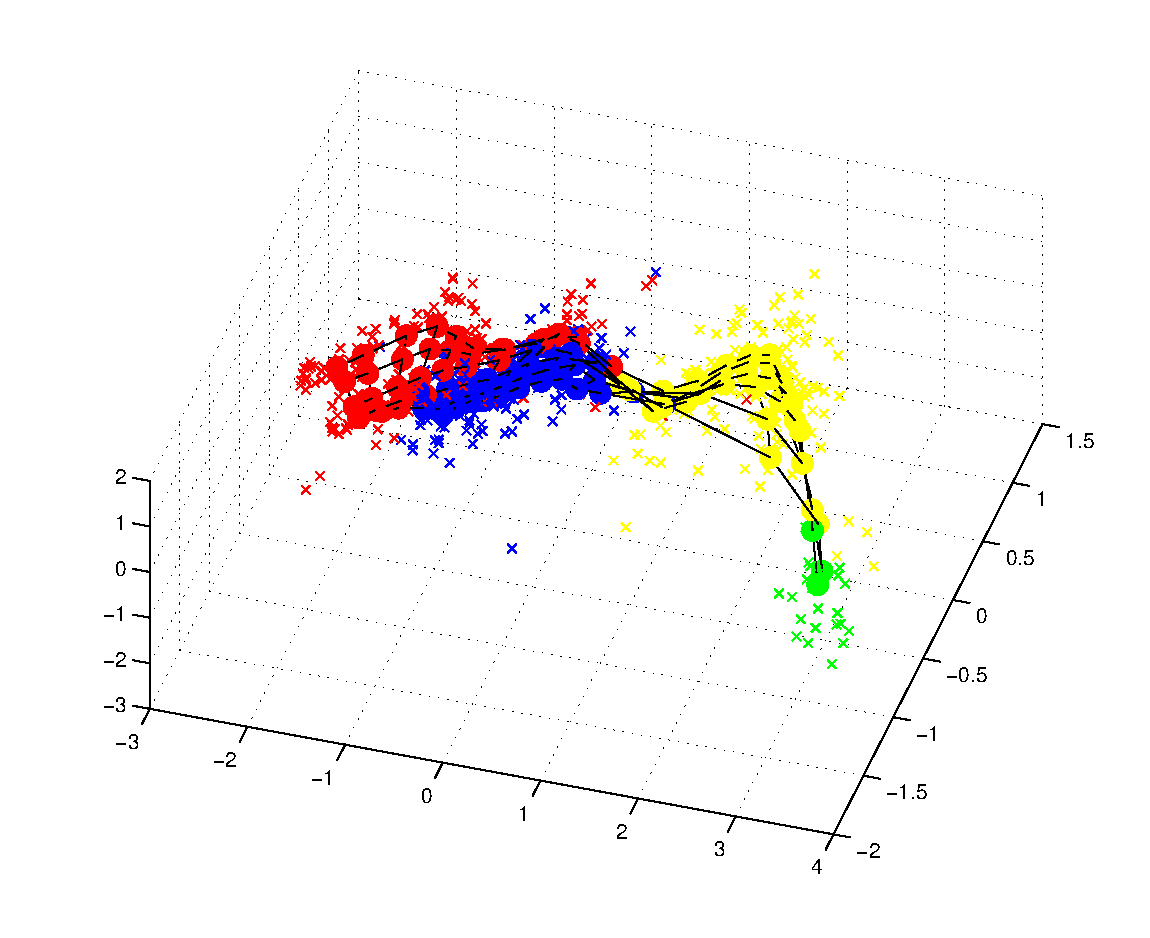
\includegraphics[width=80mm]{som_topol_proj}
\caption{Projection of topology of self-organizing map along with a data}
\label{som_topol_proj}
\end{figure}
\begin{figure}[h]
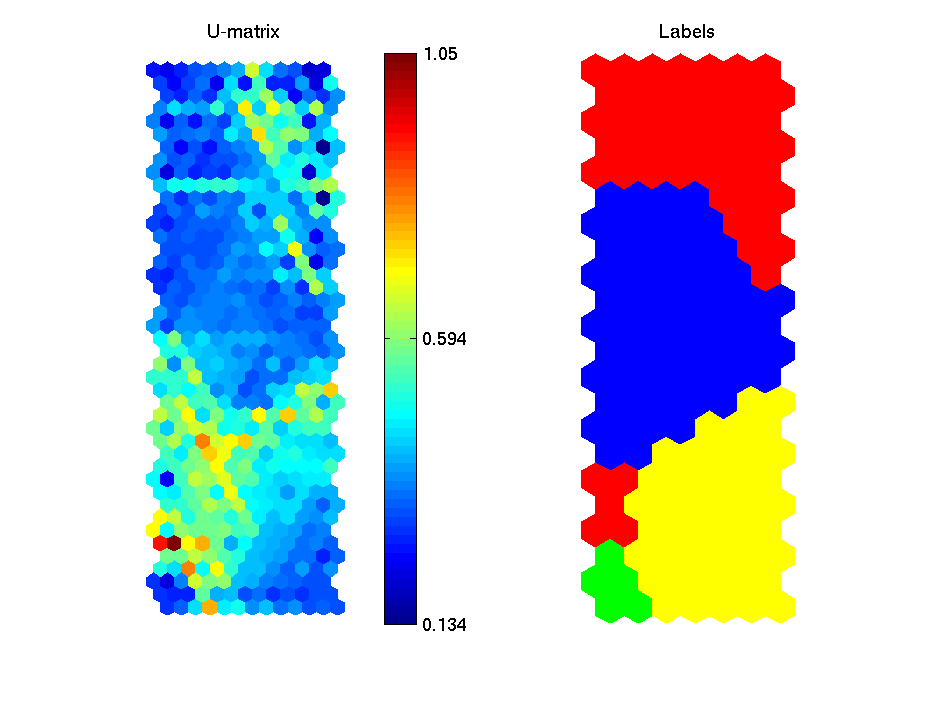
\includegraphics[width=80mm]{som_umat}
\caption{U-matrix and classification of BMUs}
\label{som_umat}
\end{figure}
Figure \ref{som_topol_proj} depicts the trained sel-organizing map and 
traning data.
Figure \ref{som_umat} shows best matching units...

\subsection{Genetic algorithm}

% if have a single appendix:
%\appendix[Proof of the Zonklar Equations]
% or
%\appendix  % for no appendix heading
% do not use \section anymore after \appendix, only \section*
% is possibly needed

% use appendices with more than one appendix
% then use \section to start each appendix
% you must declare a \section before using any
% \subsection or using \label (\appendices by itself
% starts a section numbered zero.)
%


\appendices




% trigger a \newpage just before the given reference
% number - used to balance the columns on the last page
% adjust value as needed - may need to be readjusted if
% the document is modified later
%\IEEEtriggeratref{8}
% The "triggered" command can be changed if desired:
%\IEEEtriggercmd{\enlargethispage{-5in}}

% references section

% can use a bibliography generated by BibTeX as a .bbl file
% BibTeX documentation can be easily obtained at:
% http://www.ctan.org/tex-archive/biblio/bibtex/contrib/doc/
% The IEEEtran BibTeX style support page is at:
% http://www.michaelshell.org/tex/ieeetran/bibtex/
%\bibliographystyle{IEEEtran}
% argument is your BibTeX string definitions and bibliography database(s)
%\bibliography{IEEEabrv,../bib/paper}
%
% <OR> manually copy in the resultant .bbl file
% set second argument of \begin to the number of references
% (used to reserve space for the reference number labels box)
\begin{thebibliography}{1}

\bibitem{somtoolbox}
Esa Alhoniemi, Johan Himberg, Juha Parhankangas, Juha Vesanto:
\emph{SOM Toolbox} \hskip 1em plus
  0.5em minus 0.4em\relax http://www.cis.hut.fi/projects/somtoolbox/

\bibitem{ga}
Michalewicz, Z.: 
\emph{Genetic Algorithms + Data Structures = Evolution Programs}, \hskip 1em plus
  0.5em minus 0.4em\relax Springer, 1998
  
\bibitem{gawiki}
  \emph{Genetic algorithm}, \hskip 1em plus 0.5em minus 0.4em\relax \url{http://en.wikipedia.org/wiki/Genetic_algorithms}

\end{thebibliography}

% biography section
% 
% If you have an EPS/PDF photo (graphicx package needed) extra braces are
% needed around the contents of the optional argument to biography to prevent
% the LaTeX parser from getting confused when it sees the complicated
% \includegraphics command within an optional argument. (You could create
% your own custom macro containing the \includegraphics command to make things
% simpler here.)
%\begin{biography}[{\includegraphics[width=1in,height=1.25in,clip,keepaspectratio]{mshell}}]{Michael Shell}
% or if you just want to reserve a space for a photo:



% that's all folks
\end{document}
